% !TeX spellcheck = en_US

\chapter{Extending minimal DFAs} \label{ch:4}

We firstly define a formal problem for extending a minimal DFA $A_{sol}$ to a task DFA $A_{task}$ based on our requirements analysis (see~\ref{ch:1:requirements-analysis}):
\begin{definition}[ExtendMinimalDFA] $ $ \\
	$ $ \vspace{-0.cm} \\
	\noindent $\underline{\emph{Given:}}$
	\vspace{-0.2cm}
	\begin{align*}
	A_{sol} = (Q, \Sigma, \delta, s, F) \in \Amin\ \ \ & \emph{solution DFA} \\
	\nEQ \in \mathbb{N}\ \ \ & \emph{number of states creating equivalent state pairs} \\
	\nUN \in \mathbb{N}\ \ \ & \emph{number of unreachable states} \\
	p \in \{0,1\}\ \ \ & \emph{planarity-bit} \\
	c \in \{0,1\}\ \ \ & \emph{completeness-bit}
	\end{align*}
	\noindent $\underline{\emph{Task:}}$ \emph{Compute, if it exists, a task DFA $A_{task}$ with}
	\begin{itemize}
		\item $Q_{task} = Q_{sol} \cup \{ r_1, \ldots, r_\nEQ, u_1, \ldots, u_\nUN \}$
		\item $r_1, \ldots, r_\nEQ$ \emph{each creating an equivalent state pair}
		\item $u_1, \ldots, u_\nUN$ \emph{unreachable}
		\item $\Sigma_{task} = \Sigma_{sol}$, $s_{task} = s_{sol}$, $F_{task} \subseteq F_{sol}$
		\item $A_{task}$ \emph{being planar iff} $p = 1$
		\item $A_{task}$ \emph{being complete iff} $c = 1$
		\item $A_{sol}$ \emph{being isomorph to} $\MinAlg(A_{task})$
	\end{itemize}
\end{definition}
\noindent In order to fulfill these requirements we will deduce for both kinds of states how they may be added by examining their desired properties. We will show for the action of adding equivalent states, that this does not change a DFAs $\mmD$-value.

\section{Creating equivalent state pairs}

Step 3 and 4 of the minimization algorithm are concerned with detection and elimination of equivalent state pairs. We now want to add states $r_1,\ldots,r_\nEQ$ to a DFA $A_{sol}$, gaining $A_{re}$ with $Q_{re} = Q_{sol} \cup \{r_1,\ldots,r_\nEQ\}$, such that each of these states is equivalent to a state in $A_{re}$. Note that, for reasons of clarity, we are going to abbreviate from now on $A_{re} = A$, $Q_{re} = Q$, $\sim_{A_{re}} = \sim_A$ etc.

%At this point we notice, that $A_{sol}$ is isomorph to the $\sim$-equivalence automaton (see def.~\ref{ch:1:sim-eq-dfa}). We can think 

Consider the properties $r_1,\ldots,r_\nEQ$ must have. They are equivalent to states $o_1,\ldots,o_\nEQ$ of $A$.
\[
\exists r_1,\ldots,r_\nEQ \in Q\colon\ \exists o_1,\ldots,o_\nEQ \in Q\colon\ \forall i \in [1,\nEQ] \colon\ r_i \sim_A o_i
\]
But we know also and in particular, that each of them is equivalent a state $e$ of $A_{sol}$.
\[
	\exists r_1,\ldots,r_\nEQ \in Q\colon\ \forall i \in [1,\nEQ] \colon\ \exists e \in Q_{sol}\colon\ r_i \sim_A e
\]
In our algorithm, we will choose the state $e$ for each state we add.

\subsection{Adding outgoing transitions}

Regarding the outgoing transitions of any $r_i$ equivalent to a state $e$, we are directly restricted by the relationship $\forall \sigma \in \Sigma \colon [\delta(r_i, \sigma)]_{\sim_A} = [\delta(e, \sigma)]_{\sim_A}$. Thus, when adding some $r_i$, we have to choose for each symbol $\sigma \in \Sigma$ at exactly one transition (completeness requirement for $A$) from the following set:
\[
	O_{e,\sigma} = \{\ ((r_i, \sigma), q)\ |\ q \in [\delta(e, \sigma)]_{\sim_A}\ \}
\]
Since the solution DFA is complete and since every here added state gets a transition for every alphabet symbol, we know that every $O_{e,\sigma} \neq \emptyset$.

\gregor{Why does this not affect the eq. class of any other state?}

\subsection{Adding ingoing transitions}

First of all, we know, that $r_i$ is reachable, since every state of $A$ must be reachable, so we need to give $r_i$ at least one ingoing transition. Doing this, we have to ensure, that any state $q$, that gets such an outgoing transition to $r_i$ remains in its $\sim$-equivalence class.
	
Thus a fitting state $q$ has to have a transition to some state in $[r_i]_{\sim_A} = [e]_{\sim_A}$ already. So, given a state $q$ with $\delta(q, \sigma) = p$ and $p \in [e]_{\sim_A}$, we can set $\delta(q, \sigma) = r_i$ and thus ``steal'' $q$ its ingoing transition.

We see here, that $q$ must have at least $2$ ingoing transitions, else it would become unreachable. Thus we summarize:
\[
    I_e = \{\ ((q, \sigma), p)\ |\ \delta(q, \sigma) = p \land p \in [e] \land d^-(p) \geq 2\ \}
\]
Choose at least one $((q, \sigma), p) \in I_e$, remove $((q, \sigma), p)$ from $\delta$ and add $((q, \sigma), r_i)$. 

These finding lead us to a general requirement regarding the choice of a state $e$ for an $r_i$: The equivalence class of any $e$ has to contain at least one state with at least $2$ ingoing transitions (see fig.~\ref{fig:dfa_create_equivalent_states}). We establish the following notion to pin down this restriction:
\[
	duplicatable(q) \Leftrightarrow_{def} (\exists p \in [q]_{\sim_A}\colon |d^-(p)| \geq 2)
\]
The number of duplicatable states in any accessible DFA $A$ is $0$ for $|\Sigma| \leq 1$ (due to the restriction $|d^-(p)| \geq 2$) and greater than $0$ for $|\Sigma| > 1$ due to the pigeonhole principle: An accessible complete DFA has $|Q||\Sigma|$ transitions which have to be spread across $|Q|$ states.
\begin{example}
	\begin{tikzpicture}[initial text={},scale=1., every node/.style={transform shape}]
	\tikzstyle{every state}=[minimum size=5mm, inner sep=0pt]
	
	\node[initial, state]  (03) at (0, 0)   {$03$};
	\node[state] 		   (1) at (6, 0)   {$1$};
	\node[state,accepting] (24) at (4,0)    {$24$};
	\node[state]           (6) at (2,0)    {$6$};
	
	\path[->]
	(03) edge node [above=-0.07cm]  {$a$}   (6)
	(03) edge [bend left] node [above=-0.07cm]  {$b$}   (24)
	
	(1) edge node [above=-0.13cm]  {$a,b$}   (24)
	
	(24) edge [bend left=50] node [above=-0.07cm]  {$a$}   (1)
	(24) edge [bend right=50] node [above=-0.07cm]  {$b$}   (03)
	
	(6) edge [bend right] node [below=-0.07cm]  {$a$}   (1)
	(6) edge node [above=-0.07cm]  {$b$}   (24)
	;
	\end{tikzpicture}
\end{example}
\begin{figure}
	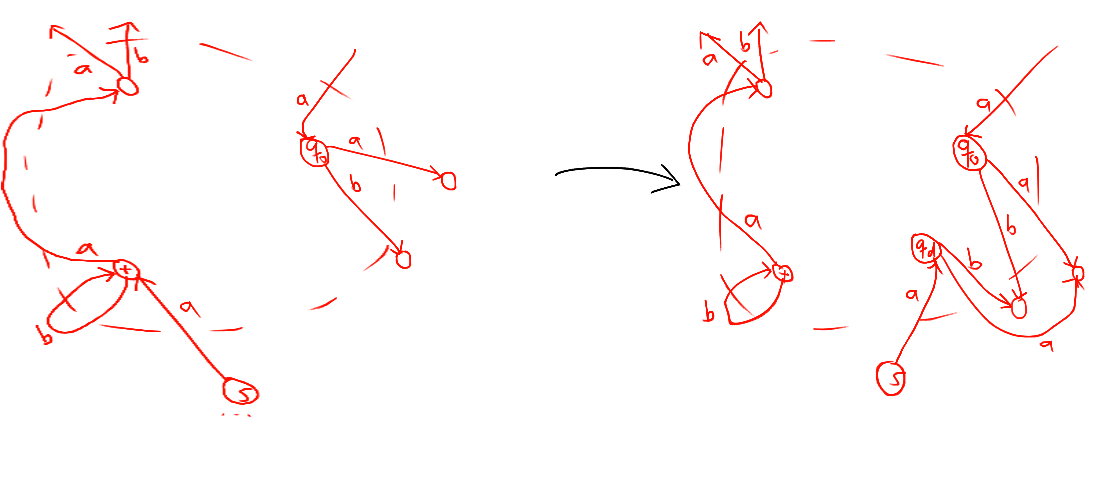
\includegraphics[width=\linewidth]{images/dfa_create_equivalent_states.png}
	\caption{If an equivalence class (here denoted by the states in the dashed area) contains a state with 2 or more ingoing transitions (in this case $p$), then a state equivalent to any of the classes states may be added. Here $r$ is equivalent to $o$ and is ``stealing'' the ingoing transition $\delta(q, a)$ from $p$.}
	\label{fig:dfa_create_equivalent_states}
\end{figure}

\subsection{The algorithm}

\vspace{0.2cm}
\begin{spacing}{1}
\begin{algorithmic}[1]
	\Function{CreateEquivalentStatePairs}{$A, \nEQ$}
    \State $Q \gets Q_{sol}$
    \State $\delta \gets \delta_{sol}$
    \State $F \gets F_{sol}$
	\State $K \gets \{\ \{q\}\ |\ q \in Q\ \}$ \Comment{tracks the equivalence classes of $A$}
	\State $k(q) = C$ such that $q \in C$ and $C \in K$ \Comment{returns the equivalence class to $q$}
	\State $in(q) = |d^-(q)|$ for all $q \in Q$ \Comment{tracks the number of ingoing t.}
	
    \For {$i$ \textbf{in} $[1,\nEQ]$}
		\For {$q$ \textbf{in} $Q$} \Comment{find a duplicatable state $e$}
			\If {$in(q) \geq 2$}
				\State $e \gets$ random chosen state from $k(q)$
				\State \textbf{break}
			\EndIf
		\EndFor
		
		\State $r_i \gets$ unused state label \Comment{create to $e$ equivalent state $r_i$}
        \State Add $r_i$ to $Q$
		\State Add $r_i$ to $k(e)$
		
		\For {$\sigma$ \textbf{in} $\Sigma$} \Comment{add $d^+(r_i)$}
			\State $\delta(r_i, \sigma) =$ random chosen state from $k(\delta(e, \sigma))$
		\EndFor
		
		\State $P \gets \{\ ((s, \sigma), t) \in \delta\ |\ t \in k(e),\ in(t) \geq 2\ \}$ \Comment{add $d^-(r_i)$}
		\State $C \gets$ random nonempty subset of $P$
		\For {$((s, \sigma), t)$ \textbf{in} $C$}
			\State $in(t) \gets in(t) - 1$
			\State $in(r_i) \gets 1$
            \State $\delta(s, \sigma) = r_i$
		\EndFor
	\EndFor
    \State \Return $(Q, \Sigma_{sol}, \delta, s_{sol}, F)$
	\EndFunction
\end{algorithmic}
\end{spacing}
\vspace{0.2cm}
\noindent Note that computing an unused state label can be easily done by e.g.\ taking the maximum of all solution DFA states (which are nothing else but numbers) and adding one.

\subsection{The existence of equivalent state pairs does not affect D} \label{ch:3:sec-D-proof}

To prove this statement, we will first introduce two auxiliary definitions and prove two minor propositions.

A word $w$ shall be called \emph{finishing word of $q$}, iff $\delta^*(q, w) \in F$. With $f(q) = \{\ w\ |\ \delta^*(q, w) \in F\ \}$ we denote the set of all finishing words to a state.
\begin{definition} \label{ch:4:def-dist-word}
	We will call a word $w$ \emph{distinguishing word of $p,q$}, iff $d_A(w, p, q)$ is true where
	\begin{align*}
	d_A(w, p, q) \text{ is true} &\Leftrightarrow (\delta^*(p,w) \in F \Leftrightarrow \delta^*(q,w) \notin F) \\
	&\Leftrightarrow (w \in f(p) \Leftrightarrow w \notin f(q))
	\end{align*}
\end{definition}
\noindent The following lemma and its proof are in parts inspired by Martens and Schwentick \cite[ch.\ 4 p.\ 18]{MS18}.

\begin{lemma}\label{ch:3:semantics-of-m(n)}
    In the context of \CompDist\ the following is true: If and only if $(p,q)\in m(n)$, the shortest distinguishing word of $p,q$ has length $n$. Formally:
    \begin{align*}
        (p,q) \in m(n) \Longleftrightarrow\ &\exists w\in\Sigma^*\colon (|w| = n\ \land d_A(w, p, q))\\
        \land\ &\nexists v\in\Sigma^*\colon (|v| < n\ \land d_A(v, p, q))
    \end{align*}
\end{lemma}

\begin{proof}
	Per induction on the number of \CompDist-iterations $n$.
	
	\paragraph*{$n = 0$, ``$\Leftrightarrow$''.}
	\begin{align*}
		&(p,q) \in m(0) = \{ (p,q), (q,p)\ |\ p \in F, q \notin F \}\hfill\text{ (see alg.~\ref{ch:1:m-minmark}, line 2))}\\
		\Leftrightarrow\ &\text{one of $p,q$ in $F$, one not}\\
		\Leftrightarrow\ &\text{one of $\delta^*(p, \varepsilon),\delta^*(q, \varepsilon)$ in $F$, one not}\\
		\Leftrightarrow\ &\exists w\in\Sigma^*\colon (|w|=0\land\text{one of $\delta^*(p, w),\delta^*(q, w)$ in $F$, one not})\\
		\Leftrightarrow\ &\exists w\in\Sigma^*\colon (|w| = 0\ \land d_A(w, p, q))\\
		&\text{and there is no shorter such word }\checkmark
	\end{align*}
	
	\paragraph*{$0\ldots n-1 \rightarrow n$, ``$\Rightarrow$''.} 
	Then the following holds for some states $p,q$ (see alg.~\ref{ch:1:m-minmark}, line 5):
	\begin{equation}\label{ch:3:eq:m(n)}
		(p,q) \in m(n) = \{ (p,q), (q,p)\ |\ (p,q) \notin \bigcup{m(\cdot)} \land \exists \sigma \in \Sigma \colon (\delta(p,\sigma), \delta(q,\sigma)) \in m(n-1) \}
	\end{equation}
	So, in particular there exists a symbol $\sigma$ such that $(\delta(p,\sigma),\delta(q,\sigma)) \in m(n-1)$. Let $(p',q')=(\delta(p,\sigma),\delta(q,\sigma))$, so $(p',q')\in m(n-1)$.
	
	Per induction there exists a shortest distinguishing word $w'$, $|w'|=n-1$ to $p',q'$. Thus one of $\delta^*(p', w'),\delta^*(q', w')$ is in $F$, one not and there is no shorter word.
	
	Thus one of $\delta^*(p, \sigma w'),\delta^*(q, \sigma w')$ is in $F$, one not, which makes $\sigma w'$ a distinguishing word of length $n$ for $p,q$.
	
	Since $(p,q)$ is not in any $m(i), i<n$ (recall $(p,q) \notin \bigcup{m(\cdot)}$ of eq.~\ref{ch:3:eq:m(n)}), there is per induction no shorter distinguishing word.\ $\checkmark$ 
	
	\paragraph*{$0\ldots n-1 \rightarrow n$, ``$\Leftarrow$''.} 
	Then the following holds for some states $p,q$:
	\begin{align*}
	&\exists w\in\Sigma^*\colon (|w| = n\ \land d_A(w, p, q))\\
	\land\ &\nexists v\in\Sigma^*\colon (|v| < |w|\ \land d_A(v, p, q))
	\end{align*}
	So there exists a word $w$ with $|w|=n>0$ such that one of $\delta^*(p, w),\delta^*(q, w)$ is in $F$, one not and there is no shorter word fulfilling this property.
	
	Since $w$ is non-empty there exists a symbol $\sigma$ such that $w = \sigma w'$. Let $(\delta(p,\sigma),\delta(q,\sigma)) = (p',q')$.
	
	Thus, if one of $\delta^*(p, \sigma w'),\delta^*(q, \sigma w')$ is in $F$ and one not, then the same must hold for $\delta^*(p', w'),\delta^*(q', w')$, so $w'$ is a distinguishing word for $p',q'$.
	
	It is also the shortest one, because, if there existed a shorter word $v'$, $|v'| < |w'|$, then $\sigma v'$ would be a distinguishing word shorter than $w$ for $p,q$ which is contradictory.
	
	Since $w'$ is a shortest distinguishing word for $p',q'$, we may deduce now per induction, that $(p',q')\in m(n-1)$.
	
	The pair $(p,q)$ is not in any $m(i)$, $i<n$, since otherwise per induction the shortest distinguishing word would be shorter than $w$ and thus not $w$. Since $(p',q')\in m(n-1)$ and $(\delta(p,\sigma),\delta(q,\sigma)) = (p',q')$, we can then deduce by the definition of $m$, that $(p,q)\in m(n)$.\ $\checkmark$ 
\end{proof}

\begin{lemma}\label{ch:3:semantics-of-D(A)}
    If \CompDist\ has done $\mmD(A)$ iterations and terminated, then the longest word $w$, that is a shortest distinguishing word for any state pair, has length $\mmD(A)-1$.
\end{lemma}

\begin{proof}
	Via direct proof. Assume $m$-\CompDist(A) has done $n$ iterations (so $\mmD(A) = n$). We observe, that
	\begin{enumerate}
		\item $\forall i \in [0,n-1]\colon m(i) \neq \emptyset$
		\item $m(n)= \emptyset$
		\item $\forall i > n\colon m(i)= \bot$\ .
	\end{enumerate}
	This follows directly from while loop and its terminating condition of \CompDist (alg.~\ref{ch:1:m-minmark}, line 4--7). Given this, we will prove: There exists a shortest distinguishing word of length $n-1$ for some state pair, but a longer such word can not exist.
    
%    Recall Lemma~\ref{ch:3:semantics-of-m(n)}:
%    \begin{align*}
%    (p,q) \in m(n) \Longleftrightarrow\ &\exists w\in\Sigma^*\colon (|w| = n\ \land d_A(w, p, q))\\
%    \land\ &\nexists v\in\Sigma^*\colon (|v| < |w|\ \land d_A(v, p, q))
%    \end{align*}

	% a possible word per definition of D(A), m(i) and lemma
	
	Following Lemma~\ref{ch:3:semantics-of-m(n)} and the first observation, we can deduce the existence of a shortest distinguishing word $w$ with $|w| = n-1 = \mmD(A)-1$ for some $p,q \in Q$.
	
	% There is no word longer than that
	
	There cannot be any shortest distinguishing word $w'$ with $|w'| = k > n-1$ for any two states $p',q'\in Q$. Following Lemma~\ref{ch:3:semantics-of-m(n)} again, $m(k)$ for some $k > n-1$ would be defined and non-empty, which is contradictory to observations 2 and 3.
\end{proof}

%\begin{lemma}\label{ch:3:lem:disting-trans}
%	If $w$ is shortest distinguishing word for $p,q$ and $q \sim_A q'$, then $w$ is a shortest distinguishing word for $p,q'$.
%%    \[
%%    d_A(w, p, q) \land q \sim_A q' \Rightarrow d_A(w, p, q')
%%    \]
%\end{lemma}
%
%\begin{proof}
%    Via direct proof. The relation $q \sim_A q'$ says that for all words $z$, $\delta^*(q,z)$ and $\delta^*(q',z)$ are both in $F$ or both not in $F$. Consequently asking whether the following is true
%    \[
%    	\delta^*(p,z)\in F \Leftrightarrow \delta^*(q,z)\in F
%    \]
%    is the same as asking whether this is true:
%    \[
%    	\delta^*(p,z)\in F \Leftrightarrow \delta^*(q',z)\in F
%    \]
%    This implies, that $q$ and $q'$ have exactly the same distinguishing words with other states (see definition of distinguishing words). As a consequence they too have the same shortest distinguishing words with other states.
%\end{proof}

\begin{theorem}
	Given two accessible DFAs $A$, $A'$. If their language is the same ($L(A) = L(A')$), then $\mmD(A) = \mmD(A')$.
\end{theorem}

\begin{proof}
	Per direct proof. Starting with the language-equivalence of $A$ and $A'$ we observe, that the start states of both DFAs have the same finishing words.
	\vspace{0.25cm}
	\begin{itemize}
		\item[] $L(A) = L(A')$
		
		\item[$\Rightarrow$] $\{\ w\ |\ \delta^*(s, w) \in F\ \} = \{\ w\ |\ \delta'^*(s', w) \in F'\ \}$
		
		\item[$\Rightarrow$] $\forall w \in \Sigma^*\colon \delta^*(s, w) \in F \Leftrightarrow \delta'^*(s', w) \in F'$
	\end{itemize}
	We extend this to a statement that includes any state visited on the way to $F$ resp.\ $F'$.
	\begin{itemize}
		\item[] $\forall u \in \Sigma^*\colon \forall v \in \Sigma^*\colon$
		
		\qquad $\delta^*(s, u) = q \land \delta'^*(s', u) = q' \land$
		
		\qquad $(\delta^*(q, v) \in F \Leftrightarrow \delta'^*(q', v) \in F')$
	\end{itemize}
	Through shifting the second quantor directly before the last line we can now see, that those states reached by the same word in $A$, $A'$ have the same finishing words.
	\begin{itemize}
		\item[] $\forall u \in \Sigma^*\colon \forall v \in \Sigma^*\colon$
		
		\qquad $\delta^*(s, u) = q \land \delta'^*(s', u) = q' \land$
		
		\qquad $(\forall v \in \Sigma^*\colon (\delta^*(q, v) \in F \Leftrightarrow \delta'^*(q', v) \in F'))$
		
		\item[$\Rightarrow$] $\forall u \in \Sigma^*\colon$
		
		\qquad $\delta^*(s, u) = q \land \delta'^*(s', u) = q' \land$
		
		\qquad $f(q) = f(q')$
	\end{itemize}
	Since we are making a statement about all states reached from $s$/$s'$ and since all states in $A$/$A'$ are reachable, we may conclude:
	
	For every state in $A$/$A'$ there exists a state in the other DFA, such that their finishing words are equal.
	\begin{itemize}
		\item [] $\forall q \in Q\colon \exists q' \in Q'\colon f(q) = f(q')$ \hfill $\land$ \hfill $\forall q' \in Q'\colon \exists q \in Q\colon f(q') = f(q)$ \qquad \qquad \qquad \qquad
		
		\item[$\Rightarrow$] $\{\ f(q)\ |\ q \in Q\ \} = \{\ f(q')\ |\ q' \in Q'\ \}$
	\end{itemize}
	Since every distinguishing word is a finishing word (see def.~\ref{ch:4:def-dist-word}), there cannot be a distinguishing word in one of $A$/$A'$, that is not distinguishing word in the other DFA.
	
	As a consequence both DFAs have the same shortest distinguishing words and thus too the same longest shortest distinguishing word.
	
	If $\mmD(A) \neq \mmD(A')$ then by Lemma~\ref{ch:3:semantics-of-D(A)} one DFA would have a longer longest shortest distinguishing word, which is not possible as proven, thus $\mmD(A) = \mmD(A')$ must be true. 
\end{proof}

\section{Adding unreachable states}

From step 1 of the minimization algorithm we can deduce how to add unreachable states. These can easily be added to a DFA by adding non-start states with no ingoing transitions (see def.~\ref{ch:1:unreachable-states}). Number and nature of outgoing transitions may be arbitrary.

\vspace{0.2cm}
\begin{algorithmic}[1]
	\Function{AddUnreachableStates\ }{$A, \nUN, c$}
	\For {$\nUN$ \textbf{times}}
		\State $q \gets$ unused state label
		\State $Q \gets Q \cup \{ q \}$
        \State $outSymbols \gets c = 1\ ?\ \Sigma\ :\ $ random subset of $\Sigma$
		\State $R \gets$ random chosen sample of $|outSymbols|$ states from $Q \setminus \{q\}$
		\For {$\sigma$ \textbf{in} $outSymbols$}
			\State $q' \in R$
			\State $R \gets R \setminus \{q'\}$
			\State $\delta \gets \delta \cup \{ ((q, \sigma), q') \}$
		\EndFor
	\EndFor
	\State \Return $A$
	\EndFunction
\end{algorithmic}
\vspace{0.2cm}
If completeness is demanded ($c=1$), then we set $\Sigma$ as set of all symbols, for which a state shall gain outgoing transitions. Else we choose a random subset for each state, such that some unreachable states may miss some outgoing transitions.
